%設定頁面
\documentclass[12pt,a4paper]{article}
\usepackage[margin=1in,a4paper]{geometry}

%設定中文
\usepackage{xeCJK} 
\setCJKmainfont{標楷體} 
\XeTeXlinebreaklocale "zh"   
\XeTeXlinebreakskip = 0pt plus 1pt 

%浮水印
%\usepackage{draftwatermark}
%\SetWatermarkText{\bf NTNU MATH}
%\SetWatermarkScale{0.7}

%圖片
\usepackage{graphicx}
\usepackage{subfigure}

%頁首頁尾
\makeatother
\usepackage{fancyhdr}

%顏色
\usepackage{xcolor}

%設定數學
\usepackage{amsmath, amsthm, amssymb}
\makeatletter

%自定圈圈標號
\usepackage{pstricks,pstricks-add}
\newcommand\textc[1]{{\begin{pspicture*}
(-0.25,-0.2)(0.25,0.3)\rput[c](0,0)
{\large \textcircled{\footnotesize #1}}
\end{pspicture*} }}

%自訂向量符號
\def\leftharpoonfill@{\arrowfill@\leftharpoonup\relbar\relbar}
\def\rightharpoonfill@{\arrowfill@\relbar\relbar\rightharpoonup}
\newcommand\rbjt{\mathpalette{\overarrow@\rightharpoonfill@}}
\newcommand\lbjt{\mathpalette{\overarrow@\leftharpoonfill@}}

%自訂定理
\newtheorem*{thm}{Theorem}
\newtheorem*{lem}{Lemma}
\newtheorem*{de}{Definition}
\newtheorem*{rmk}{Remark}
\newtheorem*{ex}{Example}
\newtheorem*{pf}{Proof}
\newtheorem*{sol}{Solution}

%程式碼
\usepackage{listings}
\usepackage{color}

\definecolor{dkgreen}{rgb}{0,0.6,0}
\definecolor{gray}{rgb}{0.5,0.5,0.5}
\definecolor{mauve}{rgb}{0.58,0,0.82}

\lstset{frame=tb,
  language=Python,
  aboveskip=3mm,
  belowskip=3mm,
  showstringspaces=false,
  columns=flexible,
  basicstyle={\small\ttfamily},
  numbers=left,
  numberstyle=\tiny\color{gray},
  keywordstyle=\color{blue},
  commentstyle=\color{dkgreen},
  stringstyle=\color{mauve},
  breaklines=true,
  breakatwhitespace=true,
  tabsize=3,
  backgroundcolor=\color{gray!10}
}




%作者
\title{NTNU影像處理HW1}
\author{廖家緯}
\date{2020.3.18}

\begin{document}
\maketitle
%標題、作者、日期
\fontsize{12pt}{20pt}\selectfont
%設定字體大小、間距
\setlength{\baselineskip}{20pt}
%設定行距

\pagestyle{fancy}
\lhead{}
\chead{}
\rhead{}
\lfoot{}
\cfoot{\thepage}
\rfoot{}
\renewcommand{\headrulewidth}{0pt} %上線寬
\renewcommand{\footrulewidth}{0pt} %下線寬
%\renewcommand{\abstractname}{Executive Summary}




%正文開始
\begin{enumerate}

\item[•]
{\bf Outline}:
\begin{enumerate}
\item
Input a color image $C(R,G,B)$.
\item
Output the color image $C$.
\item
Transform the color image C into a 
grayscale image $I$ by
$I = \displaystyle \frac{R+G+B}{3}$.
\item
Show the grayscale image $I$.\\
\end{enumerate}

\item[•]
{\bf Code(Python):}
\begin{lstlisting}
# coding: utf-8
import numpy as np
import cv2

# 讀取圖檔
img = cv2.imread('image.jpg', cv2.IMREAD_COLOR)

#提取RGB矩陣
(B, G, R) = cv2.split(img)

#取平均值,轉灰階
mean =  B/3 + G/3 + R/3
mean = np.uint8(mean)
gray_img = cv2.merge([mean, mean, mean])

# 顯示原圖
cv2.imshow('My Image', img)

# 按下任意鍵則關閉所有視窗
cv2.waitKey(0)
cv2.destroyAllWindows()

# 顯示灰階影像
cv2.imshow('My Image', gray_img)

# 按下任意鍵則關閉所有視窗
cv2.waitKey(0)
cv2.destroyAllWindows()

#儲存影像
cv2.imwrite('Original.jpg', img)
cv2.imwrite('Gray.jpg', gray_img)


\end{lstlisting}

\item[•]
{\bf Result:}

\begin{figure}[h]
\hspace*{3em}
\begin{tabular}{cc}
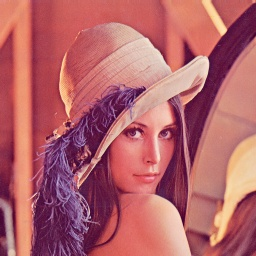
\includegraphics[height=2.4in]{Original.jpg} &
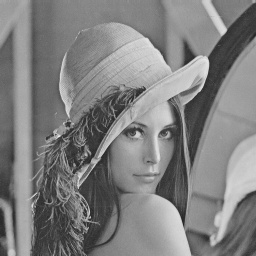
\includegraphics[height=2.4in]{Gray.jpg}\\
原圖 & 灰階
\end{tabular}
\end{figure} 

\item[•]
{\bf Experience:}\\
第一次使用Python opencv的套件,花了不少時間研究各種函式的功能。雖然有函式能夠直接將彩圖轉成灰階影像,但我還是嘗試自己找出R, G, B矩陣,再將三個矩陣的數值取平均,並轉成uint8的型態。


\end{enumerate}










\end{document}